% !TeX spellcheck = en_GB
\begin{figure}[!b]
	\centering
	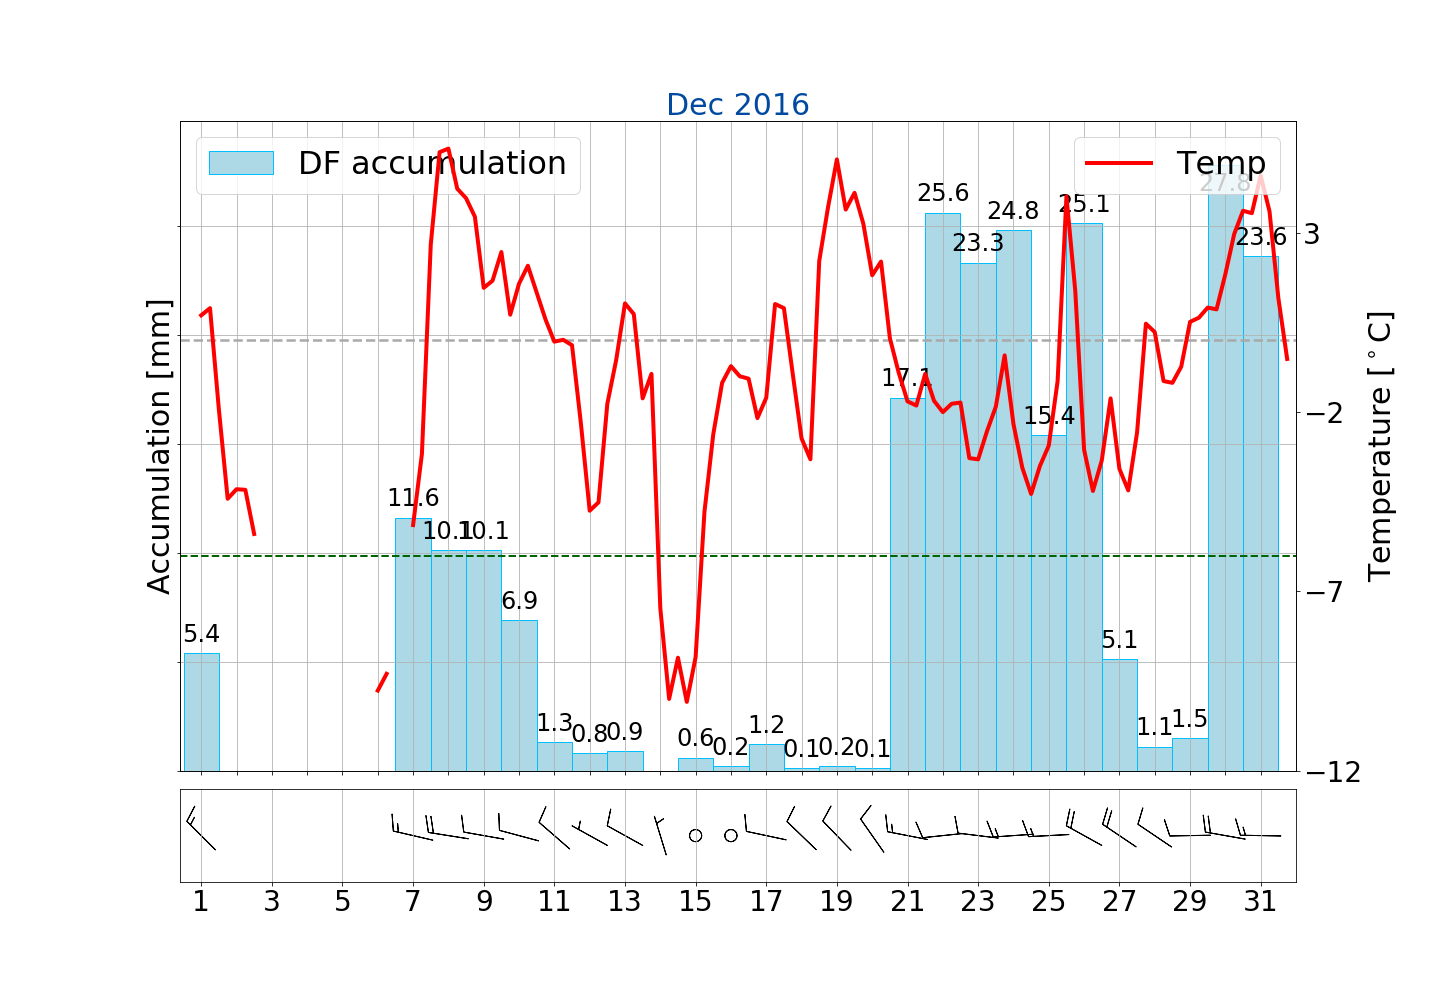
\includegraphics[trim={4.cm 3.3cm 1.5cm 3.cm},clip,
	width=0.65\textwidth]{./fig_weathermast/T_P_U_201612}
	\caption{Observations at Haukeliseter weather mast during December 2016. 
    The daily accumulation is presented in light blue [\SI{}{\mm}]; the six hour mean temperature in red, [\SI{}{\celsius}], and daily maximum \SI{10}{\metre} wind as barbs [\SI{}{\mPs}]. Gray dashed line indicates the freezing temperature. The freezing temperature is indicated by the green dashed line and the monthly normal value (\SI{-6.0}{\celsius}) by the green \citep{eklima_norwegian_2016}. Note, no data was available from \num{2} to \SI{6}{\dec}.} \label{fig:DecObs}
\end{figure}